\documentclass[draft]{beamer}
% \mode<presentation>
\setbeamertemplate{navigation symbols}{}
\let\tempone\itemize
\let\temptwo\enditemize
\renewenvironment{itemize}{\tempone\addtolength{\itemsep}{0.5\baselineskip}}{\temptwo}

\usepackage{multimedia}

\usepackage[absolute,overlay]{textpos}
\usepackage[texcoord,grid,gridunit=mm,gridcolor=red!10,subgridcolor=green!10]
{eso-pic}

%%%%%%%%%%%%%%%%%%%%%%
\usepackage{beamerthemeshadow}
\usepackage[normalem]{ulem}
\usepackage{xcolor}
\usepackage{hyperref}
\usepackage{pgffor}
\usepackage{booktabs}
\usepackage{graphicx}
\graphicspath{{figs/}}
\usepackage{amssymb}
\usepackage{bbm}
\usepackage{tabularx}
\usepackage{tikz,etoolbox}
\usepackage{tikz,amsmath,siunitx}
\usepackage{xmpmulti}


\usetikzlibrary{arrows,snakes,backgrounds,patterns,matrix,shapes,fit,calc,shadows,plotmarks}
\usepackage{subcaption}
\usepackage{pgf}
\usepackage{latexsym}
\usepackage{amsfonts}
\usepackage{amssymb}
\usepackage{amsthm}
\usepackage[noend]{algpseudocode}
\usepackage{algorithm}
\usepackage{amsmath}
\usepackage{tabularx}
\usepackage{xcolor}
\usepackage[absolute,overlay]{textpos}
\usetikzlibrary{shapes,arrows,positioning,automata,positioning,spy,matrix,scopes,chains}
\newcommand{\digs}[2]{\hphantom{999}\llap{#1}\,+\,\hphantom{999}\llap{#2}}

\def\research#1{\begin{textblock*}{50mm}(80mm,7mm)\centerline{\textcolor{white}{ \footnotesize #1}}\end{textblock*}}



\setbeamersize{text margin left=6mm}
\setbeamersize{text margin right=6mm}
\renewcommand{\insertnavigation}[1]{}
\setbeamertemplate{headline}{}
\setbeamertemplate{footline}{}
\usefonttheme{professionalfonts}
\setbeamercovered{transparent}
\mode<presentation>
\linespread{1.25}
\newcommand{\thetitle}[1]{{\begin{center}\structure{{#1}}\end{center}}}
\DeclareMathOperator{\Tr}{Tr} 
\DeclareMathOperator{\JSD}{JSD} 

\newcommand{\boldA}{\boldsymbol{A}}
\newcommand{\boldB}{\boldsymbol{B}}
\newcommand{\boldC}{\boldsymbol{C}}
\newcommand{\boldD}{\boldsymbol{D}}
\newcommand{\boldE}{\boldsymbol{E}}
\newcommand{\boldF}{\boldsymbol{F}}
\newcommand{\boldG}{\boldsymbol{G}}
\newcommand{\boldH}{\boldsymbol{H}}
\newcommand{\boldI}{\boldsymbol{I}}
\newcommand{\boldJ}{\boldsymbol{J}}
\newcommand{\boldK}{\boldsymbol{K}}
\newcommand{\boldL}{\boldsymbol{L}}
\newcommand{\boldM}{\boldsymbol{M}}
\newcommand{\boldN}{\boldsymbol{N}}
\newcommand{\boldO}{\boldsymbol{O}}
\newcommand{\boldP}{\boldsymbol{P}}
\newcommand{\boldQ}{\boldsymbol{Q}}
\newcommand{\boldR}{\boldsymbol{R}}
\newcommand{\boldS}{\boldsymbol{S}}
\newcommand{\boldT}{\boldsymbol{T}}
\newcommand{\boldU}{\boldsymbol{U}}
\newcommand{\boldV}{\boldsymbol{V}}
\newcommand{\boldW}{\boldsymbol{W}}
\newcommand{\boldX}{\boldsymbol{X}}
\newcommand{\boldY}{\boldsymbol{Y}}
\newcommand{\boldZ}{\boldsymbol{Z}}
\newcommand{\bolda}{\boldsymbol{a}}
\newcommand{\boldb}{\boldsymbol{b}}
\newcommand{\boldc}{\mathbf{c}}
\newcommand{\boldd}{\boldsymbol{d}}
\newcommand{\bolde}{\boldsymbol{e}}
\newcommand{\boldf}{\boldsymbol{f}}
\newcommand{\boldg}{\boldsymbol{g}}
\newcommand{\boldh}{\boldsymbol{h}}
\newcommand{\boldi}{\boldsymbol{i}}
\newcommand{\boldj}{\boldsymbol{j}}
\newcommand{\boldk}{\boldsymbol{k}}
\newcommand{\boldl}{\boldsymbol{l}}
\newcommand{\boldm}{\boldsymbol{m}}
\newcommand{\boldn}{\boldsymbol{n}}
\newcommand{\boldo}{\boldsymbol{o}}
\newcommand{\boldp}{\boldsymbol{p}}
\newcommand{\boldq}{\boldsymbol{q}}
\newcommand{\boldr}{\boldsymbol{r}}
\newcommand{\bolds}{\boldsymbol{s}}
\newcommand{\boldt}{\boldsymbol{t}}
\newcommand{\boldu}{\boldsymbol{u}}
\newcommand{\boldv}{\boldsymbol{v}}
\newcommand{\boldw}{\boldsymbol{w}}
\newcommand{\boldx}{\mathbf{x}}
\newcommand{\boldy}{\boldsymbol{y}}
\newcommand{\boldz}{\mathbf{z}}

\newcommand{\mcA}{\mathcal{A}}
\newcommand{\mcB}{\mathcal{B}}
\newcommand{\mcC}{\mathcal{C}}
\newcommand{\mcD}{\mathcal{D}}
\newcommand{\mcE}{\mathcal{E}}
\newcommand{\mcF}{\mathcal{F}}
\newcommand{\mcG}{\mathcal{G}}
\newcommand{\mcH}{\mathcal{H}}
\newcommand{\mcI}{\mathcal{I}}
\newcommand{\mcJ}{\mathcal{J}}
\newcommand{\mcK}{\mathcal{K}}
\newcommand{\mcL}{\mathcal{L}}
\newcommand{\mcM}{\mathcal{M}}
\newcommand{\mcN}{\mathcal{N}}
\newcommand{\mcO}{\mathcal{O}}
\newcommand{\mcP}{\mathcal{P}}
\newcommand{\mcQ}{\mathcal{Q}}
\newcommand{\mcR}{\mathcal{R}}
\newcommand{\mcS}{\mathcal{S}}
\newcommand{\mcT}{\mathcal{T}}
\newcommand{\mcU}{\mathcal{U}}
\newcommand{\mcV}{\mathcal{V}}
\newcommand{\mcW}{\mathcal{W}}
\newcommand{\mcX}{\mathcal{X}}
\newcommand{\mcY}{\mathcal{Y}}
\newcommand{\mcZ}{\mathcal{Z}}

\newcommand{\reals}{\ensuremath{\mathbb{R}}}
\newcommand{\integers}{\ensuremath{\mathbb{Z}}}
\newcommand{\rationals}{\ensuremath{\mathbb{Q}}}
\newcommand{\naturals}{\ensuremath{\mathbb{N}}}
\newcommand{\trans}{\ensuremath{\mathsf{T}}}
\newcommand{\ident}{\boldsymbol{I}}
\newcommand{\bzero}{\boldsymbol{0}}

\newcommand{\balpha}{\boldsymbol{\alpha}}
\newcommand{\bbeta}{\boldsymbol{\beta}}
\newcommand{\bdelta}{\boldsymbol{\delta}}
\newcommand{\boldeta}{\boldsymbol{\eta}}
\newcommand{\bkappa}{\boldsymbol{\kappa}}
\newcommand{\bgamma}{\boldsymbol{\gamma}}
\newcommand{\bmu}{\boldsymbol{\mu}}
\newcommand{\bphi}{\boldsymbol{\phi}}
\newcommand{\bpi}{\boldsymbol{\pi}}
\newcommand{\bpsi}{\boldsymbol{\psi}}
\newcommand{\bsigma}{\boldsymbol{\sigma}}
\newcommand{\btheta}{\boldsymbol{\theta}}
\newcommand{\bxi}{\boldsymbol{\xi}}
\newcommand{\bGamma}{\boldsymbol{\Gamma}}
\newcommand{\bLambda}{\boldsymbol{\Lambda}}
\newcommand{\bOmega}{\boldsymbol{\Omega}}
\newcommand{\bPhi}{\boldsymbol{\Phi}}
\newcommand{\bPi}{\boldsymbol{\Pi}}
\newcommand{\bPsi}{\boldsymbol{\Psi}}
\newcommand{\bSigma}{\boldsymbol{\Sigma}}
\newcommand{\bTheta}{\boldsymbol{\Theta}}
\newcommand{\bUpsilon}{\boldsymbol{\Upsilon}}
\newcommand{\bXi}{\boldsymbol{\Xi}}
\newcommand{\bepsilon}{\boldsymbol{\epsilon}}

\def\argmin{\operatornamewithlimits{arg\,min}}
\def\argmax{\operatornamewithlimits{arg\,max}}

\newcommand{\given}{\,|\,}
\newcommand{\param}{; \,}

\newcommand{\distNorm}{\mathcal{N}}

\newcommand{\E}{\mathbb{E}}
\newcommand{\ind}{\mathbb{1}}
\newcommand{\Hess}{\mathrm{H}}
\DeclareMathOperator*{\KL}{KL}
\DeclareMathOperator*{\ELBO}{ELBO}
\DeclareMathOperator*{\RELU}{ReLU}
\DeclareMathOperator*{\MLP}{MLP}
\DeclareMathOperator*{\LSTM}{LSTM}
\DeclareMathOperator*{\RNN}{RNN}
\DeclareMathOperator*{\RNNLM}{RNNLM}
\DeclareMathOperator*{\softmax}{softmax}
\DeclareMathOperator*{\enc}{enc}
\DeclareMathOperator*{\gen}{gen}
\DeclareMathOperator*{\sal}{sal}
\DeclareMathOperator*{\encsal}{input-sal}
\DeclareMathOperator*{\clip}{clip}


\usepackage{color}
\usepackage{blindtext}
\usepackage{multirow}
\usepackage{rotating}
\usepackage[all,dvips]{xy}
\usepackage{colortbl}
\usepackage{graphicx}
\usepackage{verbatim}
\usepackage{framed}
\usepackage{natbib}
\usepackage[labelformat=empty]{caption}
\newcommand{\air}{\vspace{0.25cm}}
\newcommand{\mair}{\vspace{-0.25cm}}

\setbeamertemplate{navigation symbols}{}%remove navigation symbols
\renewcommand{\rmdefault}{crm}
\definecolor{vermillion}{RGB}{213,94,0}
\definecolor{orange}{RGB}{230,159,0}
\definecolor{skyblue}{RGB}{86,180,233}
\definecolor{bluegreen}{RGB}{90,143,41}
% \definecolor{bluegreen}{RGB}{0,158,115}
\definecolor{myyellow}{RGB}{240,228,66} % i dunno if this is the same as standard yellow
\definecolor{myblue}{RGB}{0,114,178}
\definecolor{vermillion}{RGB}{213,94,0}
\definecolor{redpurple}{RGB}{204,121,167}
\definecolor{lightgrey}{RGB}{234,234,234}
\usepackage{tikz}
\usetikzlibrary{fit,positioning}
\usetikzlibrary{bayesnet}
\usetikzlibrary{arrows}
\usetikzlibrary{decorations.pathreplacing}
% \setbeamerfont{alerted text}{series=\bfseries}
% \setbeamerfont{structure}{series=\bfseries}
% Needed for diakgrams.
\def\im#1#2{
  \node(#1) [scale=#2]{\pgfbox[center,top]{\pgfuseimage{#1}}
};}
% \input{pictures_header}
% make smaller citations
\let\realcitep\citep
\renewcommand*{\citep}[1]{{\scriptsize \realcitep{#1}}}
\let\realcitet\citet
\renewcommand*{\citet}[1]{{\scriptsize \realcitet{#1}}}
\setcitestyle{square,semicolon,aysep={}}

%%%%%%%%%%%%%%%%%%%%%%%%%%%%%%%%%%%%%%%%%%%%%%%%%%%%

\title[]{Text Generation }
\author[]{Alexander Rush}
\institute[Harvard SEAS]{
  % \begin{center}
  %   \includegraphics[width=5cm]{harvardnlp}
  % \end{center}
  \vspace{0.5cm}
  {\Large }\\

  { }
}

%%%%%%%%%%%%%%%%%%%%%%%%%%%%%%%%%%%%%%%%%%%%%
\makeatletter
\long\def\beamer@@frametitle[#1]#2{%
  \beamer@ifempty{#2}{}{%
    \gdef\insertframetitle{\centering{#2\ifnum\beamer@autobreakcount>0\relax{}\space\usebeamertemplate*{frametitle continuation}\fi}}%
  \gdef\beamer@frametitle{#2}%
  \gdef\beamer@shortframetitle{#1}%
}%
}
\makeatother
%%%%%%%%%%%%%%%%%%%%%%%%%%%%%%%%%%%%%%%%%%%%%

\date{}
%\usetheme{Madrid}
\usetheme[hideothersubsections]{Singapore}
\definecolor{darkgreen}{rgb}{0.13, 0.55, 0.13}
\definecolor{darkpurple}{rgb}{0.55, 0.0, 0.55}

\AtBeginSection[]
{
  \begin{frame}
  \tableofcontents[currentsection,hideothersubsections]
  \end{frame}
}

\AtBeginSubsection[]
{
  \begin{frame}
  \tableofcontents[currentsection,
        currentsubsection,
        subsectionstyle=show/shaded/hide]
  \end{frame}
}


\def\argmax{\operatornamewithlimits{arg\,max}}
\def\kargmax{\operatornamewithlimits{K-arg\,max}}
\setbeamercovered{transparent}


\begin{document}
\maketitle

\section{Introduction}


\begin{frame}

  % Application pictures
\end{frame}

\begin{frame}{Text Generation}

  \[ \argmax_{y_{1:T}} f(y_{1:T} ; x, \theta)\]

\end{frame}

\begin{frame}{Natural Language Processing, 2009}

  % Picture
  \begin{tikzpicture}
    \node{};
  \end{tikzpicture}

\end{frame}

\begin{frame}{Natural Language Processing, 2019}

  % Picture
  \begin{tikzpicture}
    \node{};
  \end{tikzpicture}

\end{frame}

\begin{frame}{Performance}

\end{frame}


\begin{frame}

\end{frame}

\begin{frame}{Central}
  % Picture
  \begin{tikzpicture}
    \node{};
  \end{tikzpicture}
\end{frame}


\begin{frame}{My Research}{}
  % Picture
  \research{\cite{Deng2016}}


  \begin{tikzpicture}
    \node{};
  \end{tikzpicture}
\end{frame}


\begin{frame}{My Research}{}
  % Pictured






  \begin{center}
  \begin{tikzpicture}

    \node at (-35mm, 15mm) {
      \scriptsize
      \citet{Kim2016}
      };
    \node[draw] (ana) at (-15mm, 15mm) {Analysis};
    \node[draw] (meth) at (0mm, 30mm) {\ Methods\phantom{p}};
    \node at (0mm, 40mm) {
      \scriptsize
      \citet{Kim2016}
      };

    \node[draw] (app) at (25mm, 30mm) {Applications};
    \node at (25mm, 40mm) {
      \scriptsize
      \citet{Kim2016}
      };



    \node[draw] (und) at (35mm, 15mm) {Understanding};


    \node at (60mm, 15mm) {
      \scriptsize
      \citet{Kim2016}
      };


    \node[draw] (dep) at (25mm, 0mm){Deployment};

    \node at (25mm, -10mm) {
      \scriptsize
      \citet{Kim2016}
      };

    \node[draw] (imp) at (0, 0) {Development};

      \node at (0mm, -10mm) {
      \scriptsize
      \citet{Kim2016}
      };


    \draw (ana) -- (meth) --(app) -- (und) -- (dep) -- (imp) -- (ana);

  \end{tikzpicture}
  \end{center}
\end{frame}


\section{Section 1}


\begin{frame}{Section 1: Analysis and Development}

\end{frame}


\begin{frame}{Autoregressive Neural Networks}
\multiinclude[format=png,start=1,graphics={width=\textwidth}]{figs/nmt-noattn}
\end{frame}


\begin{frame}{Autoregressive Neural Networks Math}
  \movie[height=6.5cm, width=6.5cm]{Temporary}{flame.avi}
\end{frame}

\begin{frame}{LSTMVis}
  \research{\citet{Strobelt2016} w/ IBM}
  \movie[height=6.5cm, width=6.5cm]{Temporary}{flame.avi}

  (LSTM Video)


\end{frame}

\begin{frame}{Seq2Seq Model}
  \multiinclude[format=png,start=1,graphics={width=\textwidth}]{figs/nmt-attn}
\end{frame}

\begin{frame}{Seq2SeqVis}
  \research{\citet{strobelt2019s} w/ IBM}

  
\end{frame}


\begin{frame}{OpenNMT}
  \includegraphics[width=\textwidth]{opennmtpanaram.jpg}
\end{frame}


\section{Section 2: Applications}
\begin{frame}
  \begin{center}
    \textbf{The Modern Text Generation Challenge} 
  \end{center}
  \begin{center}
\begin{tikzpicture}
\node{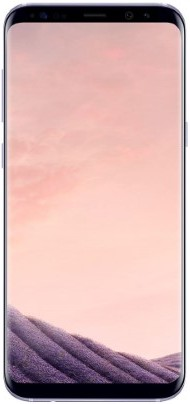
\includegraphics[width=5cm]{galaxy}};
\end{tikzpicture}
  \end{center}
\end{frame}

% \begin{frame}
%   \begin{center}
%     \structure{The Modern Text Generation Challenge: \\ Make Some Conversation (Chatbots)} 
%   \end{center}
%   \begin{center}
% \begin{tikzpicture}
% \node{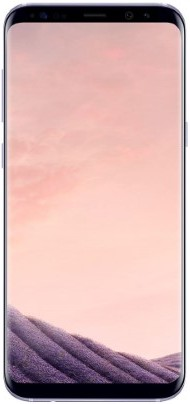
\includegraphics[width=5cm]{galaxy}};
% \path[draw] (0, 0) --  (2,0) ;
% \node [xshift=3.5cm, rectangle, draw,thick,fill=blue!0,text width=8em, rounded corners, inner sep =5pt, minimum height=1em]{\baselineskip=50pt \footnotesize Hi there Joe, have a good day today!  \par};
% \end{tikzpicture}
%   \end{center}
% \end{frame}


\begin{frame}{Talk about Text (Summarization) }

  \research{\citet{Rush2015} w/ Facebook}


  \begin{center}
\begin{tikzpicture}
\node{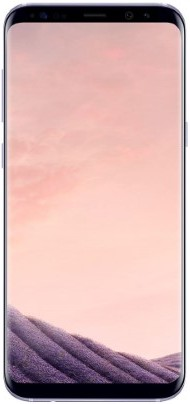
\includegraphics[width=5cm]{galaxy}};
\path<2>[draw] (0, 0) --  (2,0) ;

\node[inner sep=1pt, rounded corners, text width=15em, xshift=-4cm,]{\small

\vspace{0.5cm}
\tiny
mexico city , mexico -lrb- cnn -rrb- -- heavy rains and flooding have forced hundreds of thousands of people from homes in southern mexico 's state of tabasco over the past four days , with nearly as many trapped by the rising waters , state officials said thursday . officials say about 300,000 people are still trapped by the worst flooding in the region for 50 years . the grijalva river pushed over its banks through the state capital of villahermosa on thursday , forcing government workers to evacuate and leaving up to 80 percent of the city flooded , gov. andres granier 's office told cnn . about 700,000 people have seen their homes flooded , with about 300,000 of those still trapped there , granier 's office reported . one death had been blamed on the floods , which followed weeks of heavy rain in the largely swampy state . tabasco borders guatemala to the south and the gulf of mexico to the north . \ldots

};
\visible<2>{
\node [xshift=3.5cm, rectangle, draw,thick,fill=blue!0,text width=8em, rounded corners, inner sep =5pt, minimum height=1em]{\baselineskip=50pt \footnotesize tabasco and chiapas states hardest hit. authorities say 700,000 affected \ldots   \par};}
\end{tikzpicture}
  \end{center}
\end{frame}

\begin{frame}{Summarization}
  
\end{frame}


\begin{frame}{Talk about Information (Generation) } 

  \research{\cite{EMNLP2017}}
  \begin{center}
\begin{tikzpicture}
\node{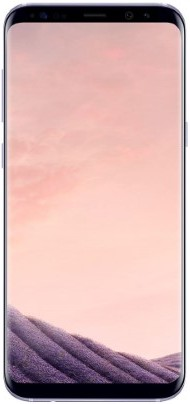
\includegraphics[width=5cm]{galaxy}};
\path<2>[draw] (0, 0) --  (2,0) ;
\node[inner sep=1pt, rounded corners, text width=15em, xshift=-4cm,]{\small
  \begin{center}
\vspace{0.5cm}
\footnotesize
\begin{tabular}{lcccccc}
\toprule
{} & W & L & PTS &  \ldots \\
TEAM &           &             &          &                      \\
\midrule
Heat   &        11 &          12 &      103 &     \ldots      \\
Hawks  &         7 &          15 &       95 &     \ldots      \\
\bottomrule

\vspace*{0.3cm}
\end{tabular}

% \begin{tabular}{lccccccccc}
% \toprule
% {} &  AS &    RB &   PT &  FG &  FGA & CITY  $\ldots$ \\
% PLAYER      &      &      &      &       &      &      &           \\
% \midrule
% Tyler Johnson    &    5 &    2 &  27 &    8 &   16 &     Miami \\
% Dwight Howard    &    11 &    17 &  23 &    9 &   11 &   Atlanta \\
% Paul Millsap     &    2 &    9 &  21 &    8 &   12 &   Atlanta \\
% Goran Dragic     &    4 &    2 &  21 &    8 &   17 &     Miami \\
% Wayne Ellington  &    2 &    3 &  19 &    7 &   15 &     Miami \\
% Dennis Schroder  &    7 &    4 &  17 &    8 &   15 &   Atlanta \\
% Rodney McGruder  &    5 &    5 &  11 &    3 &    8 &     Miami \\
% \ldots \\
% \bottomrule
% \end{tabular}

  \end{center}




};
 % \node [xshift=-3.5cm, rectangle, draw,thick,fill=blue!0,text width=8em, rounded corners, inner sep =5pt, minimum height=1em]{\baselineskip=50pt \footnotesize The Atlanta Hawks defeated the Miami Heat, 103 - 95, at Philips Arena on Wednesday. Atlanta  ... \par};
\visible<2>{\node[xshift=3.5cm, rectangle, draw,thick,fill=blue!0,text width=8em, rounded corners, inner sep =5pt, minimum height=1em]{\baselineskip=50pt \footnotesize The Atlanta Hawks defeated the Miami Heat, 103 - 95, at Philips Arena on Wednesday. Atlanta  ... \par};}
\end{tikzpicture}
  \end{center}
\end{frame}


\begin{frame}
  \begin{center}
    \textbf{Case Study: Data-to-Document Generation}
  \end{center}

\vspace{-0.7cm}
  \begin{figure}
\centering
\scalebox{0.6}{
\begin{tikzpicture}
\node[draw, inner sep=10pt, rounded corners, text width=30em, xshift=-7.5cm,]{\small
  \begin{center}


\begin{tabular}{lcccccc}
\toprule
{} & WIN & LOSS & PTS & FG\_PCT & RB & AS \ldots \\
TEAM &           &             &          &             &          &          \\
\midrule
Heat      &        11 &          12 &      103 &          49 &       47 &       27 \\
Hawks     &         7 &          15 &       95 &          43 &       33 &       20 \\
\bottomrule
\end{tabular}
\vspace{0.5cm}

\begin{tabular}{lccccccccc}
\toprule
{} &  AS &    RB &   PT &  FG &  FGA & CITY  $\ldots$ \\
PLAYER      &      &      &      &       &      &      &           \\
\midrule
Tyler Johnson    &    5 &    2 &  27 &    8 &   16 &     Miami \\
Dwight Howard    &    11 &    17 &  23 &    9 &   11 &   Atlanta \\
Paul Millsap     &    2 &    9 &  21 &    8 &   12 &   Atlanta \\
Goran Dragic     &    4 &    2 &  21 &    8 &   17 &     Miami \\
Wayne Ellington  &    2 &    3 &  19 &    7 &   15 &     Miami \\
Dennis Schroder  &    7 &    4 &  17 &    8 &   15 &   Atlanta \\
Rodney McGruder  &    5 &    5 &  11 &    3 &    8 &     Miami \\
\ldots \\
\bottomrule
\end{tabular}

  \end{center}

};


\node [yshift=-4cm, rectangle, draw,thick,fill=blue!0,text width=30em, rounded corners, inner sep =10pt, minimum height=1em]{\baselineskip=100pt \large  The Atlanta Hawks defeated the Miami Heat, 103 - 95, at Philips Arena on Wednesday. Atlanta was in desperate need of a win and they were able to take care of a shorthanded Miami team here. Defense was key for the Hawks, as they held the Heat to 42 percent shooting and forced them to commit 16 turnovers. Atlanta also dominated in the paint, winning the rebounding battle, 47 - 34, and outscoring them in the paint 58 - 26. The Hawks shot 49 percent from the field and assisted on 27 of their 43 made baskets. This was a near wire-to-wire win for the Hawks, as Miami held just one lead in the first five minutes. Miami ( 7 - 15 ) are as beat-up as anyone right now and it's taking a toll on the heavily used starters. Hassan Whiteside really struggled in this game, as he amassed eight points, 12 rebounds and one blocks on 4 - of - 12 shooting ... \par};
\end{tikzpicture}
}
\caption{\small Document generation example. Left, a source consisting of structured data, in this case statistics from a basketball game. Right, a target document utilizing a select subset of records from the data,
  expressed in an often complex and expressive manner. This example is an excerpt from the case-study data set, which include
  628 records in total and a longer target document. }
\label{fig:samplesummary}
\end{figure}

\end{frame}



\begin{frame}{Talk about the Environment (Multimodal) } 
\research{\cite{Deng2016 w/ Bloomberg}}
  \begin{center}
\begin{tikzpicture}
\node{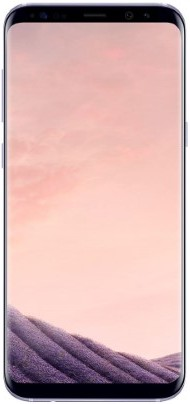
\includegraphics[width=5cm]{galaxy}};
\path<2>[draw] (0, 0) --  (2,0) ;
 \node [xshift=-4cm, rectangle, thick,fill=blue!0,text width=5cm, rounded corners, inner sep =5pt, minimum height=1em]{\baselineskip=50pt \includegraphics[width=5cm]{dowjones}};
\visible<2>{
\node [xshift=3.5cm, rectangle, draw,thick,fill=blue!0,text width=8em, rounded corners, inner sep =5pt, minimum height=1em]{\baselineskip=50pt \footnotesize Dow and S\&P 500 close out week at all-time highs ... \par};}
\end{tikzpicture}
  \end{center}
\end{frame}


\begin{frame}{Im2Latex}
  \multiinclude[format=png,start=100,graphics={width=\textwidth}]{figs/recognition}
\end{frame}
  

\section{Section 3: Structured Modeling }


\begin{frame}

\end{frame}


\begin{frame}{Application: }

\end{frame}


\section{Current Work: Deep Latent Variable Modeling}


\begin{frame}

\end{frame}

\begin{frame}

\end{frame}

\section{Impact and Outreach}

\begin{frame}{OpenNMT}

\end{frame}

\begin{frame}{LSTMVis}

\end{frame}



\section{Future Work}

\begin{frame}{Probabilistic Programming}

\end{frame}

\begin{frame}{Probabilistic Programming}

\end{frame}


\begin{frame}

\end{frame}

\bibliography{me}
\bibliographystyle{acl_natbib_nourl}

\end{document}